\section{Simulator for the C++ program}

To help create a faster development process, for the Sailing Robot project, the creation of a simulator would be useful, in the testing of the \gls{C++} program used to control the boat. 
There is some simulator to test the algorithm and Matlab but the conversion from Matlab to C++ can induce some bugs that were not yet easy to identify.
The current design of the code at the time of the creation of the simulator was too complicated and old to be able to simply implement the simulation in the code itself, therefore the easiest way to do it was to pre-empt the connection to the sensor needed to drive the boat.

\begin{figure}[H]
\centering
\psscalebox{0.5 0.5} % Change this value to rescale the drawing.
{
% \usepackage[usenames,dvipsnames]{pstricks}
% \usepackage{epsfig}
% \usepackage{pst-grad} % For gradients
% \usepackage{pst-plot} % For axes
% \usepackage[space]{grffile} % For spaces in paths
% \usepackage{etoolbox} % For spaces in paths
% \makeatletter % For spaces in paths
% \patchcmd\Gread@eps{\@inputcheck#1 }{\@inputcheck"#1"\relax}{}{}
% \makeatother
% % User Packages:
% \usepackage{amsmath}
% \usepackage{amsfonts}
% \usepackage{amssymb}
% \usepackage{algorithm}
% \usepackage{algorithmic}
\psscalebox{1.0 1.0} % Change this value to rescale the drawing.
{
\begin{pspicture}(0,-4.398276)(16.057339,4.398276)
\definecolor{colour0}{rgb}{0.65882355,0.99607843,0.35686275}
\definecolor{colour1}{rgb}{0.42352942,0.8784314,0.9764706}
\definecolor{colour2}{rgb}{0.9490196,0.5764706,0.5921569}
\psellipse[linecolor=black, linewidth=0.012, linestyle=dashed, dash=0.17638889cm 0.10583334cm, dimen=outer](7.031034,-1.3086208)(3.0275862,2.689655)
\psellipse[linecolor=black, linewidth=0.04, fillstyle=solid,fillcolor=colour0, dimen=outer](1.854732,-1.6375979)(1.583172,0.8379661)
\rput{6.7314534}(0.37274778,-0.6346489){\psellipse[linecolor=black, linewidth=0.04, fillstyle=solid,fillcolor=colour1, dimen=outer](5.5820684,2.8517241)(4.02,1.03)}
\rput{18.753927}(0.70229614,-3.9860935){\psellipse[linecolor=black, linewidth=0.04, fillstyle=solid,fillcolor=colour2, dimen=outer](12.42028,0.13337229)(1.8921099,2.7825892)}
\psline[linecolor=black, linewidth=0.04, arrowsize=0.05291667cm 2.0,arrowlength=1.4,arrowinset=0.0]{<->}(13.57026,-2.8102677)(13.243397,-1.9115297)
\rput[bl](11.606252,-3.1447155){Remote PC Control}
\rput[bl](12.480103,-1.7166519){Xbee}
\psline[linecolor=black, linewidth=0.04, arrowsize=0.05291667cm 2.0,arrowlength=1.4,arrowinset=0.0]{<->}(12.382069,-1.649387)(8.717011,-1.7143679)
\rput[bl](0.0,-2.964253){\textbf{TCP/IP Communication}}
\rput[bl](0.67349714,-1.7868472){WebServer}
\psline[linecolor=black, linewidth=0.04, arrowsize=0.05291667cm 2.0,arrowlength=1.4,arrowinset=0.0]{<->}(2.6210194,-1.6705922)(5.202069,-1.6582758)
\rput[bl](4.0903444,4.1182756){\textbf{I$^2$C Communication}}
\rput[bl](11.2173395,2.923399){\textbf{Serial Port Communication}}
\rput[bl](3.1420686,2.6217241){Pressure Sensor}
\psline[linecolor=black, linewidth=0.04, arrowsize=0.05291667cm 2.0,arrowlength=1.4,arrowinset=0.0]{->}(3.8220687,2.221724)(5.8420687,-0.17827587)
\rput[bl](11.319171,-0.44599622){Motor Controllor}
\psline[linecolor=black, linewidth=0.04, arrowsize=0.05291667cm 2.0,arrowlength=1.4,arrowinset=0.0]{<->}(11.245878,-0.48970443)(8.711275,-1.4573234)
\rput[bl](11.18373,0.52905947){Windsensor}
\psline[linecolor=black, linewidth=0.04, arrowsize=0.05291667cm 2.0,arrowlength=1.4,arrowinset=0.0]{->}(11.224926,0.5702956)(8.577307,-0.78335524)
\rput[bl](7.4620686,3.0017242){Compass}
\psline[linecolor=black, linewidth=0.04, arrowsize=0.05291667cm 2.0,arrowlength=1.4,arrowinset=0.0]{->}(7.5820684,2.7417243)(7.3420687,0.24172413)
\rput[bl](11.263345,1.9251283){GPS}
\psline[linecolor=black, linewidth=0.04, arrowsize=0.05291667cm 2.0,arrowlength=1.4,arrowinset=0.0]{->}(11.182069,1.9017241)(9.023218,0.5121456)
\rput[bl](5.8620687,-1.6782758){Main Program}
\pscircle[linecolor=black, linewidth=0.04, dimen=outer](6.9620686,-1.5382758){1.78}
\rput[bl](7.382758,-4.398276){\textit{Computing Unit}}
\psline[linecolor=black, linewidth=0.04, arrowsize=0.05291667cm 2.0,arrowlength=1.4,arrowinset=0.0]{->}(8.676984,0.12884279)(8.280845,-0.39293915)
\rput[bl](7.965766,0.2254468){{\small GPSD Daemon}}
\end{pspicture}
}


}
\caption{Data transfer model of the boat.}
\label{fig:model_boat_com}
\end{figure}

As seen on~\ref{fig:model_boat_com}, the data goes from and to the main program regulating the boat via three different means of communication.
The sensor data comes from serial ports \gls{RS232} and \gls{i2c} communication and the program send data to the remote web server via \gls{TCPIP}. The simulator only need to deal with two of the communication path, \gls{i2c} and serial communication, as the web server will always be available. 

\gls{linux} allow creating easily many virtual serial ports via programming but it is not possible to do the same for \gls{i2c} communication. To remedy at this problem the solution is to bypass function used by the main program to discuss with the I$^2$C bus. The program use a dynamic library (not compiled inside the program  and loaded in memory at runtime), functions can be overloaded if other functions with the same prototype (same name, same input parameters and same output) are loaded before. Then those function will communicate with the exterior of the program with \gls{sharedmemory}.

\begin{figure}[H]
\centering
\psscalebox{0.5 0.5} % Change this value to rescale the drawing.
{
% \usepackage[usenames,dvipsnames]{pstricks}
% \usepackage{epsfig}
% \usepackage{pst-grad} % For gradients
% \usepackage{pst-plot} % For axes
% \usepackage[space]{grffile} % For spaces in paths
% \usepackage{etoolbox} % For spaces in paths
% \makeatletter % For spaces in paths
% \patchcmd\Gread@eps{\@inputcheck#1 }{\@inputcheck"#1"\relax}{}{}
% \makeatother
% % User Packages:
% \usepackage{amsmath}
% \usepackage{amsfonts}
% \usepackage{amssymb}
% \usepackage{algorithm}
% \usepackage{algorithmic}
\psscalebox{1.0 1.0} % Change this value to rescale the drawing.
{
\begin{pspicture}(0,-4.3745584)(16.869757,4.3745584)
\definecolor{colour0}{rgb}{0.99607843,0.16470589,0.16470589}
\definecolor{colour5}{rgb}{0.99607843,0.99607843,0.99607843}
\definecolor{colour1}{rgb}{0.65882355,0.99607843,0.35686275}
\definecolor{colour2}{rgb}{0.9490196,0.5764706,0.5921569}
\definecolor{colour3}{rgb}{0.79607844,0.7607843,0.24705882}
\definecolor{colour4}{rgb}{0.6627451,0.25490198,0.63529414}
\psellipse[linecolor=black, linewidth=0.04, fillstyle=vlines, hatchwidth=0.02, hatchangle=22.0, hatchsep=0.4, hatchcolor=colour0, dimen=outer](8.260985,2.9066384)(1.6181818,1.2121212)
\psframe[linecolor=colour5, linewidth=0.04, fillstyle=solid,fillcolor=colour5, dimen=outer](9.34314,3.2042816)(7.0468435,2.4931705)
\rput{-33.63478}(1.1742575,4.476236){\psellipse[linecolor=black, linewidth=0.012, linestyle=dashed, dash=0.17638889cm 0.10583334cm, dimen=outer](7.99201,0.29558465)(3.9300253,4.396972)}
\rput{-330.17743}(-0.2676209,-1.0106432){\psellipse[linecolor=black, linewidth=0.04, fillstyle=solid,fillcolor=colour1, dimen=outer](1.7638229,-1.0078198)(1.5165052,1.3591782)}
\rput{18.753927}(0.18432017,-4.216627){\psellipse[linecolor=black, linewidth=0.04, fillstyle=solid,fillcolor=colour2, dimen=outer](12.859304,-1.5502272)(1.0433294,0.39234522)}
\psline[linecolor=black, linewidth=0.04, arrowsize=0.05291667cm 2.0,arrowlength=1.4,arrowinset=0.0]{<->}(13.57026,-2.7865503)(13.243397,-1.8878121)
\rput[bl](11.606252,-3.120998){Remote PC Control}
\rput[bl](12.480103,-1.6929344){Xbee}
\psline[linecolor=black, linewidth=0.04, arrowsize=0.05291667cm 2.0,arrowlength=1.4,arrowinset=0.0]{<->}(12.382069,-1.6256695)(8.717011,-1.6906502)
\rput[bl](0.0,-2.9405355){\textbf{TCP/IP Communication}}
\rput[bl](0.67349714,-1.7631297){WebServer}
\psline[linecolor=black, linewidth=0.04, arrowsize=0.05291667cm 2.0,arrowlength=1.4,arrowinset=0.0]{<->}(2.6210194,-1.6468747)(5.202069,-1.6345583)
\rput[bl](12.029757,-0.96005267){\textbf{Serial Port Communication}}
\rput[bl](5.7583647,-1.7138176){Main Program}
\pscircle[linecolor=black, linewidth=0.04, dimen=outer](6.9620686,-1.5145583){1.78}
\rput[bl](7.382758,-4.3745584){\textit{Computing Unit}}
\psline[linecolor=black, linewidth=0.04, arrowsize=0.05291667cm 2.0,arrowlength=1.4,arrowinset=0.0]{->}(8.676984,0.15256032)(8.280845,-0.3692216)
\rput[bl](7.965766,0.24916434){{\small GPSD Daemon}}
\psline[linecolor=colour3, linewidth=0.04, linestyle=dashed, dash=0.17638889cm 0.10583334cm, arrowsize=0.05291667cm 2.0,arrowlength=1.4,arrowinset=0.0]{->}(9.624621,2.203608)(11.345834,0.5793657)(8.570076,-0.7782101)
\psline[linecolor=colour3, linewidth=0.04, linestyle=dashed, dash=0.17638889cm 0.10583334cm, arrowsize=0.05291667cm 2.0,arrowlength=1.4,arrowinset=0.0]{<->}(8.667046,-0.9963919)(11.903409,0.5793657)(9.806439,2.6036081)
\psline[linecolor=colour3, linewidth=0.04, linestyle=dashed, dash=0.17638889cm 0.10583334cm, arrowsize=0.05291667cm 2.0,arrowlength=1.4,arrowinset=0.0]{->}(8.630682,1.7308809)(8.71553,0.61572933)
\rput[bl](1.1640154,-0.4024525){Simulator}
\psline[linecolor=black, linewidth=0.04, arrowsize=0.05291667cm 2.0,arrowlength=1.4,arrowinset=0.0]{<->}(6.679167,2.7005777)(1.7943184,0.082395986)
\rput{-44.561977}(1.2363315,7.8739686){\rput[bl](10.226605,2.428315){\small{Motor Controller}}}
\rput{-41.194386}(1.1743914,6.7127047){\rput[bl](9.517955,1.7939111){\small{Windsensor}}}
\rput{-85.93802}(6.6179576,10.209451){\rput[bl](8.789066,1.5524297){\small{GPS}}}
\rput{77.81638}(5.4495893,-6.1740537){\rput[bl](6.54947,0.28886062){\scriptsize{Pressure Sensor}}}
\rput{76.49165}(6.109742,-6.8746214){\rput[bl](7.415733,0.43835557){\small{Compass}}}
\psline[linecolor=colour4, linewidth=0.06, linestyle=dotted, dotsep=0.10583334cm, arrowsize=0.05291667cm 2.0,arrowlength=1.4,arrowinset=0.0]{->}(7.2157326,2.2028)(6.672029,-0.2105333)
\psline[linecolor=colour4, linewidth=0.06, linestyle=dotted, dotsep=0.10583334cm, arrowsize=0.05291667cm 2.0,arrowlength=1.4,arrowinset=0.0]{->}(7.8335104,1.9583555)(7.279436,-0.32016295)
\psline[linecolor=colour4, linewidth=0.06, linestyle=dotted, dotsep=0.10583334cm, arrowsize=0.05291667cm 2.0,arrowlength=1.4,arrowinset=0.0]{->}(16.157822,1.8314756)(12.598345,1.8346128)
\psline[linecolor=colour3, linewidth=0.04, linestyle=dashed, dash=0.17638889cm 0.10583334cm, arrowsize=0.05291667cm 2.0,arrowlength=1.4,arrowinset=0.0]{->}(16.090996,3.0593288)(12.557545,3.0620859)
\rput[bl](13.239436,3.2190964){Virtual Serial Port}
\rput[bl](13.491288,1.9450222){Shared Memory}
\rput[bl](7.216541,2.6736417){Side Program}
\psellipse[linecolor=black, linewidth=0.04, fillstyle=vlines, hatchwidth=0.02, hatchangle=22.0, hatchsep=0.4, hatchcolor=colour0, dimen=outer](7.0246215,-0.16608886)(0.7777778,0.36296296)
\end{pspicture}
}


}
\caption{Data transfer model of the boat with simulator.}
\label{fig:model_boat_sim}
\end{figure}

The implementation of the simulator need a program on the same computing unit as the main program to be able to use virtual serial ports and \gls{sharedmemory}, this side program is used as a proxy for the simulator, the communication is via \gls{TCPIP} to allow easy configuration (i.e.\ changing parameters of the simulation on a computer and the main program running on the embedded computer allowing to test the code directly on the computer that will be sailing).
The data transferred between the simulator and the side program are raw values, the side program will 
then transform the data for serial port as the real sensor messages, e.g.\ \gls{NMEA} messages for the GPS and 
wind sensor.

The main program was then refactor to a node and message program, meaning each sensor is a node sending messages to the node that will compute the orders to give to the actuators. The program created before work without changes on this model, but to follow the model of the program a simulation as been created, the node directly send the messages inside the program and is still discussing with the simulator with \gls{TCPIP}.
The advantage of this simulation is a simpler initialisation but the first implementation still has some assets such as allowing testing different preprocessing of data (filters).

In the end this simulator is useful as it helps the programmer test quickly the code and the implementation of the algorithm without doing real test, this should make the people gain a high amount of time.



\section{Smith predictor}

When testing a new controller, the algorithm is not implemented in the main program but a remote program will take control of the boat via an xBee (see~\ref{fig:model_boat_com}) communicating with another xBee on a remote pc on the boat following the sailboat. The xBee is managed by LabView and allow using a Matlab script to compute the command to give to the sailboat.

This communication in the current state show a delay on the actuators around 2-3 seconds and can disturb the control algorithm.

To solve this problem the use of a Smith predictor (~\cite{smith1959controller}) is proposed :

\begin{figure}[H]
\centering
\psscalebox{0.5 0.5} % Change this value to rescale the drawing.
{
% \usepackage[usenames,dvipsnames]{pstricks}
% \usepackage{epsfig}
% \usepackage{pst-grad} % For gradients
% \usepackage{pst-plot} % For axes
% \usepackage[space]{grffile} % For spaces in paths
% \usepackage{etoolbox} % For spaces in paths
% \makeatletter % For spaces in paths
% \patchcmd\Gread@eps{\@inputcheck#1 }{\@inputcheck"#1"\relax}{}{}
% \makeatother
% % User Packages:
% \usepackage{amsmath}
% \usepackage{amsfonts}
% \usepackage{amssymb}
% \usepackage{algorithm}
% \usepackage{algorithmic}
\psscalebox{1.0 1.0} % Change this value to rescale the drawing.
{
\begin{pspicture}(0,-4.1751976)(14.16,4.1751976)
\psframe[linecolor=black, linewidth=0.04, dimen=outer](12.612632,3.5100658)(9.352632,2.150066)
\psframe[linecolor=black, linewidth=0.04, dimen=outer](8.732163,-0.4449049)(5.8777776,-1.5849049)
\psframe[linecolor=black, linewidth=0.04, dimen=outer](12.053947,-0.48046044)(10.213947,-1.5404605)
\pscircle[linecolor=black, linewidth=0.04, dimen=outer](13.711579,-1.0104605){0.44842106}
\psframe[linecolor=black, linewidth=0.04, dimen=outer](4.7357893,1.6437501)(1.6557895,0.5037501)
\rput[bl](10.027632,2.6750658){Real System}
\rput[bl](6.244971,-1.169905){Model system}
\rput[bl](10.858948,-1.1454605){$e^{-\tau}$}
\rput[bl](13.884662,-0.5287311){+}
\rput[bl](13.0323305,-0.9236183){-}
\rput[bl](0.90803826,-2.7845752){+}
\rput[bl](2.4207895,0.9537501){Controller}
\pscircle[linecolor=black, linewidth=0.04, dimen=outer](0.44842106,-2.9257236){0.44842106}
\psline[linecolor=black, linewidth=0.04](9.284682,-1.008455)(9.274156,-2.9455705)
\psline[linecolor=black, linewidth=0.04, arrowsize=0.05291667cm 2.0,arrowlength=1.4,arrowinset=0.0]{->}(12.06,-1.0183551)(13.281053,-1.0078288)
\psline[linecolor=black, linewidth=0.04](13.716842,-1.4499341)(13.706316,-4.134145)
\psline[linecolor=black, linewidth=0.04](13.724689,-4.155197)(0.4705263,-4.155197)
\psline[linecolor=black, linewidth=0.04, arrowsize=0.05291667cm 2.0,arrowlength=1.4,arrowinset=0.0]{->}(9.266753,-2.9257238)(0.8657416,-2.9257238)
\psline[linecolor=black, linewidth=0.04](12.586316,2.835329)(13.730468,2.8248026)
\psline[linecolor=black, linewidth=0.04, arrowsize=0.05291667cm 2.0,arrowlength=1.4,arrowinset=0.0]{->}(13.711578,2.8132238)(13.711578,-0.55870605)
\psline[linecolor=black, linewidth=0.04](4.7740393,1.0342764)(5.4799604,1.0237501)
\psline[linecolor=black, linewidth=0.04, arrowsize=0.05291667cm 2.0,arrowlength=1.4,arrowinset=0.0]{->}(5.504015,2.8218338)(9.344211,2.8246408)
\psline[linecolor=black, linewidth=0.04, arrowsize=0.05291667cm 2.0,arrowlength=1.4,arrowinset=0.0]{->}(0.46694785,1.0790131)(1.6470436,1.0684868)
\psline[linecolor=black, linewidth=0.04](0.45368418,1.081932)(0.44315788,-2.4529963)
\psline[linecolor=black, linewidth=0.04, arrowsize=0.05291667cm 2.0,arrowlength=1.4,arrowinset=0.0]{<-}(0.448421,-3.3826613)(0.448421,-4.175197)
\psline[linecolor=black, linewidth=0.04](5.522584,2.809662)(5.5007653,-1.0303378)
\psline[linecolor=black, linewidth=0.04, arrowsize=0.05291667cm 2.0,arrowlength=1.4,arrowinset=0.0]{->}(5.514503,-1.0149047)(5.870867,-1.0149047)
\psline[linecolor=black, linewidth=0.04, arrowsize=0.05291667cm 2.0,arrowlength=1.4,arrowinset=0.0]{->}(8.717331,-1.0104607)(10.231674,-1.0104607)
\rput[bl](0.5771292,-3.6463935){+}
\rput[bl](10.813948,-0.22230256){\textit{Delay}}
\rput[bl](4.938947,0.6151974){\textit{u}}
\rput[bl](12.688948,2.9151974){$\begin{bmatrix}
    x \\
   y \\
    \theta
\end{bmatrix}$}
\rput[bl](8.922147,-0.76667035){$\begin{bmatrix}
    x_m \\
   y _m\\
    \theta_m
\end{bmatrix}$}
\psline[linecolor=black, linewidth=0.04, arrowsize=0.05291667cm 2.0,arrowlength=1.4,arrowinset=0.0]{->}(2.4029074,2.4736652)(2.4029074,1.660762)
\rput[bl](1.473875,2.6026974){\textit{Line to Follow}}
\end{pspicture}
}


}
\caption{Model Smith predictor for the sailboat}
\label{fig:smith_pred}
\end{figure}

The smith predictor (figure~\ref{fig:smith_pred}) is active on the value $x$, $y$ $\theta$  because  that is the value used by the controller. When controlling the real systems, alongside it we compute a model of the system and delay it the amount of the delay the real system seem to have. The present value is kept as the it will keep the value fed to the controller to diverge if the model is too far from reality.

A delay is created inside a Matlab simulation and the Smith predictor implemented, the real part of simulation is updating via Runge-Kutta with a 0.01 step and the model part of the simulation is integrated via Euler with 0.1 step:

\begin{figure}[H]
\centering
    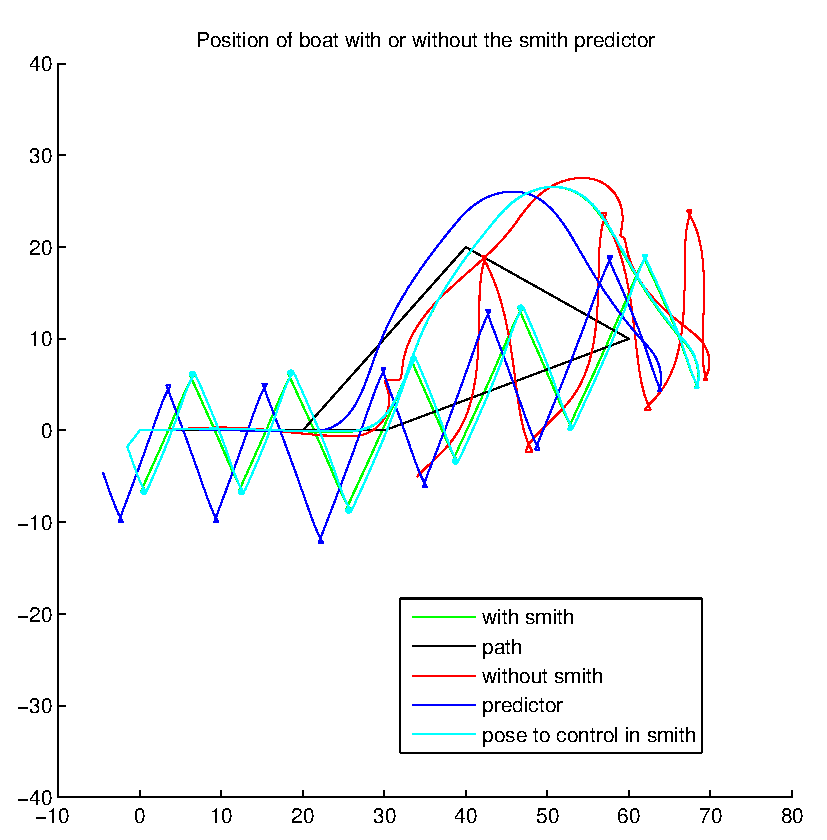
\includegraphics[scale=0.5,angle=0]{smith_predictor_pos}
    \caption{Position of the boat following a path with or without the smith predictor.}
    \label{fig:smith_predictor_pos}
\end{figure}


In the simulation \footnote{To see simulations : \href{https://www.youtube.com/watch?v=P2E160nLPyo}{Smith predictor video https://www.youtube.com/watch?v=P2E160nLPyo}} the boat without Smith predictor is slower and less precise when following the lines.
The smith predictor is effective here but, real test need to be done , to determine the efficiency of the model to predict the boat and the effect of time varying delay in the communication.

